% !TeX spellcheck = russian-aot
%\documentclass[12pt,a4paper,draft]{article}
%\usepackage{cmap}
%\usepackage[utf8]{inputenc}
%\usepackage[T2A]{fontenc}
%\usepackage[english,german,russian]{babel}
%\usepackage{amsmath}
%\usepackage{amsfonts}
%\usepackage{amssymb}
%\usepackage[final]{graphicx}
%\DeclareGraphicsExtensions{.jpg,.png}
%\graphicspath{{pictures/}} % путь к графическим файлам. Пусть они помещаются в подкаталог pictures текущего каталога
%\usepackage[figurename=Рисунок,labelsep=period]{caption}
%\usepackage{float}
%\usepackage{indentfirst}
%\usepackage[pdftex,left=2.5cm,right=2.5cm,top=3cm,bottom=3cm]{geometry}
%\usepackage[obeyDraft]{todonotes}
%\usepackage[hidelinks,draft=false]{hyperref}
%\frenchspacing
%\pdfcompresslevel=9

\documentclass[a4paper,12pt]{article}
\usepackage[utf8]{inputenc}
\usepackage[T2A]{fontenc}
\usepackage[english,russian]{babel}
\usepackage{natbib}
\usepackage[final]{graphicx}
\DeclareGraphicsExtensions{.jpg,.png}
\graphicspath{{pictures/}}
\usepackage{float}
\usepackage{amsmath}
\usepackage{pgfplots}
\usepackage{color} %% это для отображения цвета в коде
%\usepackage{listings} %% собственно, это и есть пакет listings




%\setmonofont{Consolas} %to be used with XeLaTeX or LuaLaTeX
\definecolor{bluekeywords}{rgb}{0,0,1}
\definecolor{greencomments}{rgb}{0,0.5,0}
\definecolor{redstrings}{rgb}{0.64,0.08,0.08}
\definecolor{xmlcomments}{rgb}{0.5,0.5,0.5}
\definecolor{types}{rgb}{0.17,0.57,0.68}

\usepackage{listings}
\lstset{
language=[Sharp]C,
captionpos=t,
%numbers=left, %Nummerierung
%numberstyle=\tiny, % kleine Zeilennummern
frame=lines, % Oberhalb und unterhalb des Listings ist eine Linie
showspaces=false,
showtabs=false,
breaklines=true,
showstringspaces=false,
breakatwhitespace=true,
escapeinside={(*@}{@*)},
commentstyle=\color{greencomments},
morekeywords={partial, var, value, get, set},
keywordstyle=\color{bluekeywords}\bf,
stringstyle=\color{redstrings},
basicstyle=\ttfamily\small,
extendedchars=\true
}

\usepackage{caption}
\DeclareCaptionFont{white}{\color{white}} %% это сделает текст заголовка белым
%% код ниже нарисует серую рамочку вокруг заголовка кода.
\DeclareCaptionFormat{listing}{\colorbox{gray}{\parbox{\textwidth}{#1#2#3}}}
\captionsetup[lstlisting]{format=listing,labelfont=white,textfont=white}


\usepackage{ctable}%для таблиц
\captionsetup[table]{justification=raggedleft,singlelinecheck=off}




%%%%%%%%%%%%%%%%%%%%%%%%%%%%%%%%%%%%%%%%%%%%%%%%%%%%%%%%%%%%%%%%%%%%%%%%%%%%%%%%%%%%%%%%%%%%%%%

\begin{document}
\begin{titlepage}
	\centering
    \begin{figure}[H]
    	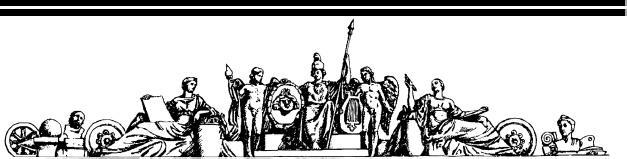
\includegraphics[scale=1.2]{photo}
   	\end{figure}
	{\scshape Министерство образования Российской Федерации
Московский Государственный Технический Университет им. Н.Э. Баумана \par}
	\vspace{4cm}
	{\scshape\Large Отчёт по лабораторной работе № 1\par}
    {\scshape\Large По курсу: "Анализ алгоритмов"\par}
	{\scshape\Large\bf Тема:"Умножение матриц. Многопоточное умножение матриц"\par}
    \vspace{2cm}
    {\flushright Студент: Орехова Е.О. ИУ7-51\par
    \flushright Преподаватель: Волкова Л.Л.\par}
    \vspace{2cm}
% Bottom of the page
	{\large \today\par}
\end{titlepage}

\def\contentaname{Содержание}
\tableofcontents %Вывод содержания
\clearpage

\section{Постановка задачи}
    В ходе выполнения лабораторной работы необходимо реализовать умножение матриц n потоками. Сравнить с однопоточной реализацией.

\section{Умножение матриц}
    Пусть даны две матрицы, $A$ и $B$, размерности $a \times n$ и $n \times b$ соответственно, тогда результатом их умножения будет матрица $C$, размерности $a \times b$, в которой
    \begin{equation}
    	C_{i,j} = \sum_{k = 1}^{n} A_{i,k}*B{k,j}
    \end{equation}
\section{Алгоритм Винограда}
	Если посмотреть на результат умножения двух матриц, то видно, что каждый элемент в нем представляет собой скалярное произведение соответствующих строки и столбца исходных матриц. Можно заметить также, что такое умножение допускает предварительную обработку, позволяющую часть работы выполнить заранее. Рассмотрим два вектора $V = (v_1,v_2,v_3,v_4)$ и $W = (w_1,w_2,w_3,w_4)$. Их скалярное произведение равно 
	\begin{equation}
		V*W = v_1w_1 + v_2w_2 + v_3w_3 + v_4w_4
	\end{equation}
	Это равенство можно переписать в виде:
	\begin{equation}
	V*W = (v_1+w_2)(v_2+w_1)+(v_3+w_4)(v_4+w_3)-v_1v_2-v_3v_4-w_1w_2-w_3w_4
	\end{equation}
	Из этого следует, что произведение матриц можно выполнить эффективнее, произведя некоторые вычисления заранее.
	
    
\section{Реализация однопоточного умножения матриц}
\begin{lstlisting}[label=some-code,caption={Стандартный алгоритм умножения матриц}]
public static void Simple_Multiplication(ref int[,]C, int[,] A, int[,] B, int size)
{
	for (int i = 0; i < size; i++)
		for (int j = 0; j < size; j++)
		{
			C[i, j] = 0;
			for (int k = 0; k < size; k++)
				C[i, j] = C[i, j] + A[i,k] * B[k,j];
		}
}
\end{lstlisting}

\begin{lstlisting}[label=some-code1,caption={Алгоритм Винограда}]
public static void Vinograd(ref int[,] C,int[,] A, int[,] B, int size, int [] Rows, int [] Column)
{
	
	for (int i = 0; i < size; i++)
	{
		Rows[i] = A[i, 0] * A[i, 1];
		for (int j = 1; j < size/2; j++)
			Rows[i] = Rows[i]+ A[i, 2 * j] * A[i, 2 * j + 1];
	}
	
	
	for (int i = 0; i < size; i++)
	{
		Column[i] = B[0, i] * B[1, i];
		for (int j = 1; j < size/2; j++)
			Column[i] = Column[i]+ B[2 * j, i] * B[2 * j + 1, i];
	}
	
	
	for(int i = 0; i< size; i++)
		for (int j = 0; j<size;j++)
		{
			C[i, j] = -Rows[i] - Column[j];
			for (int k = 0; k < size/2; k++)
				C[i, j] = C[i, j]+(A[i,2*k+1]+B[2*k,j]) * (A[i,2*k]+B[2*k+1,j]);
		}
	if (size % 2 == 1)
	{
		for (int i = 0; i < size; i++)
			for (int j = 0; j < size; j++)
				C[i, j] = C[i, j]+ A[i,size-1] * B[size-1,j];
	}
}
\end{lstlisting}

\section{Реализация многопоточного умножения матриц}
\begin{lstlisting}[label=some-code,caption={Класс для описания многопоточного умножения}]
class Simple_Multiply
{
private int begin;
private int end;
private int c;
private int b;

public Simple_Multiply(int b, int c, int begin, int end)
{
	this.begin = begin;
	this.end = end;
	this.c = c;
	this.b = b;
}

public void Simple_Multiply_Thread()
{
	for (int i = begin; i < end; i++)
		for (int j = 0; j < c; j++)
		{
			Program.D[i, j] = 0;
			for (int k = 0; k < b; k++)
				Program.D[i, j] += Program.A[i, k] *Program.B[k, j];
		}
}

public void Vinograd_Multiply_Thread()
{
	for (int i = begin; i < end; i++)
		for (int j = 0; j < c; j++)
		{
			Program.D[i, j] = -Multiplication.Rows[i] - Multiplication.Column[j];
			for (int k = 0; k < b / 2; k++)
				Program.D[i, j] += (Program.A[i, 2 * k + 1] + Program.B[2 * k, j]) * (Program.A[i, 2 * k] + Program.B[2 * k + 1, j]);
		}
		if (b % 2 == 1)
		{
		for (int i = begin; i < end; i++)
			for (int j = 0; j < c; j++)
				Program.D[i, j] += Program.A[i,b - 1] * Program.B[b - 1, j];
		}
}
}
\end{lstlisting}

\section{Эксперимент}
В проводимом эксперименте задача разбивалась на 2 потока. Умножение матриц двумя потоками происходит быстрее в независимости от количества элементов.
\begin{figure}[H]
	\noindent\centering{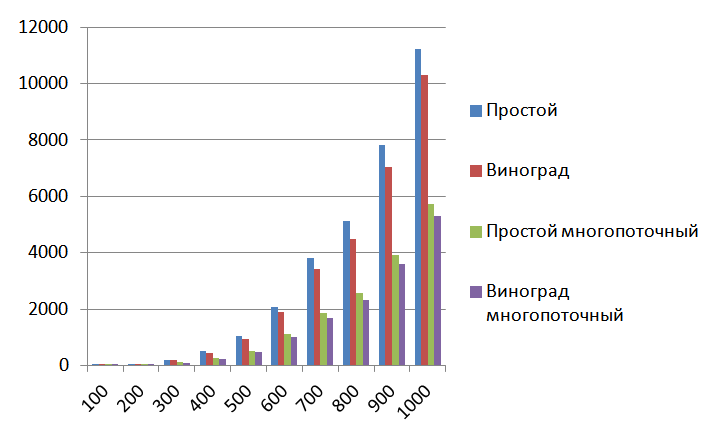
\includegraphics[scale = 1]{twothread}}
	\caption{Время умножения матриц в мс.}
\end{figure}

\begin{figure}[H]
	\noindent\centering{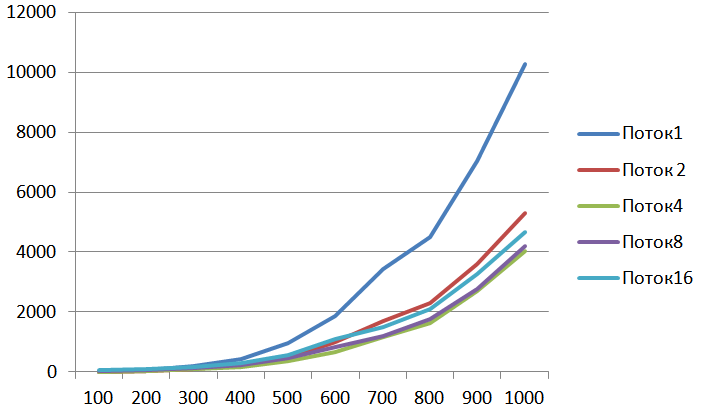
\includegraphics[scale = 1]{nthread}}
	\caption{Время умножения матриц в мс.}
\end{figure}

Оптимальное число потоков: 4-8.

\section{Заключение}
	В ходе выполнения лабораторной работы были изучены и реализованы различные алгоритмы умножения матриц. Реализовано умножение матриц средствами n потоков. Экспериментально подтверждено, что большое число потоков не всегда работает быстрее.
\end{document} 